\documentclass{article}
\usepackage{amsmath}
\usepackage{graphicx}
\begin{document}
\title{Dilations: Question 19}
\author{Ana Bhattacharjee}
\date{\today}
\maketitle{}


\begin{center}
In order to prove that the dilation takes a line passing through the center of the dilation to the same line, we must first visualize the image with respect to the pre-image after the dilation has been performed.
\begin{align}
  A(-2,2), B(1,2), C(1, -1) \\
  D_{O, 2.5} \rightarrow A,B,C = A' (-5, 5), B' (\frac{5}{2}, 5), C' (\frac{5}{2}, - \frac{5}{2})
\end{align}
The graphic is shown below.
\begin{figure}[!htbp]
  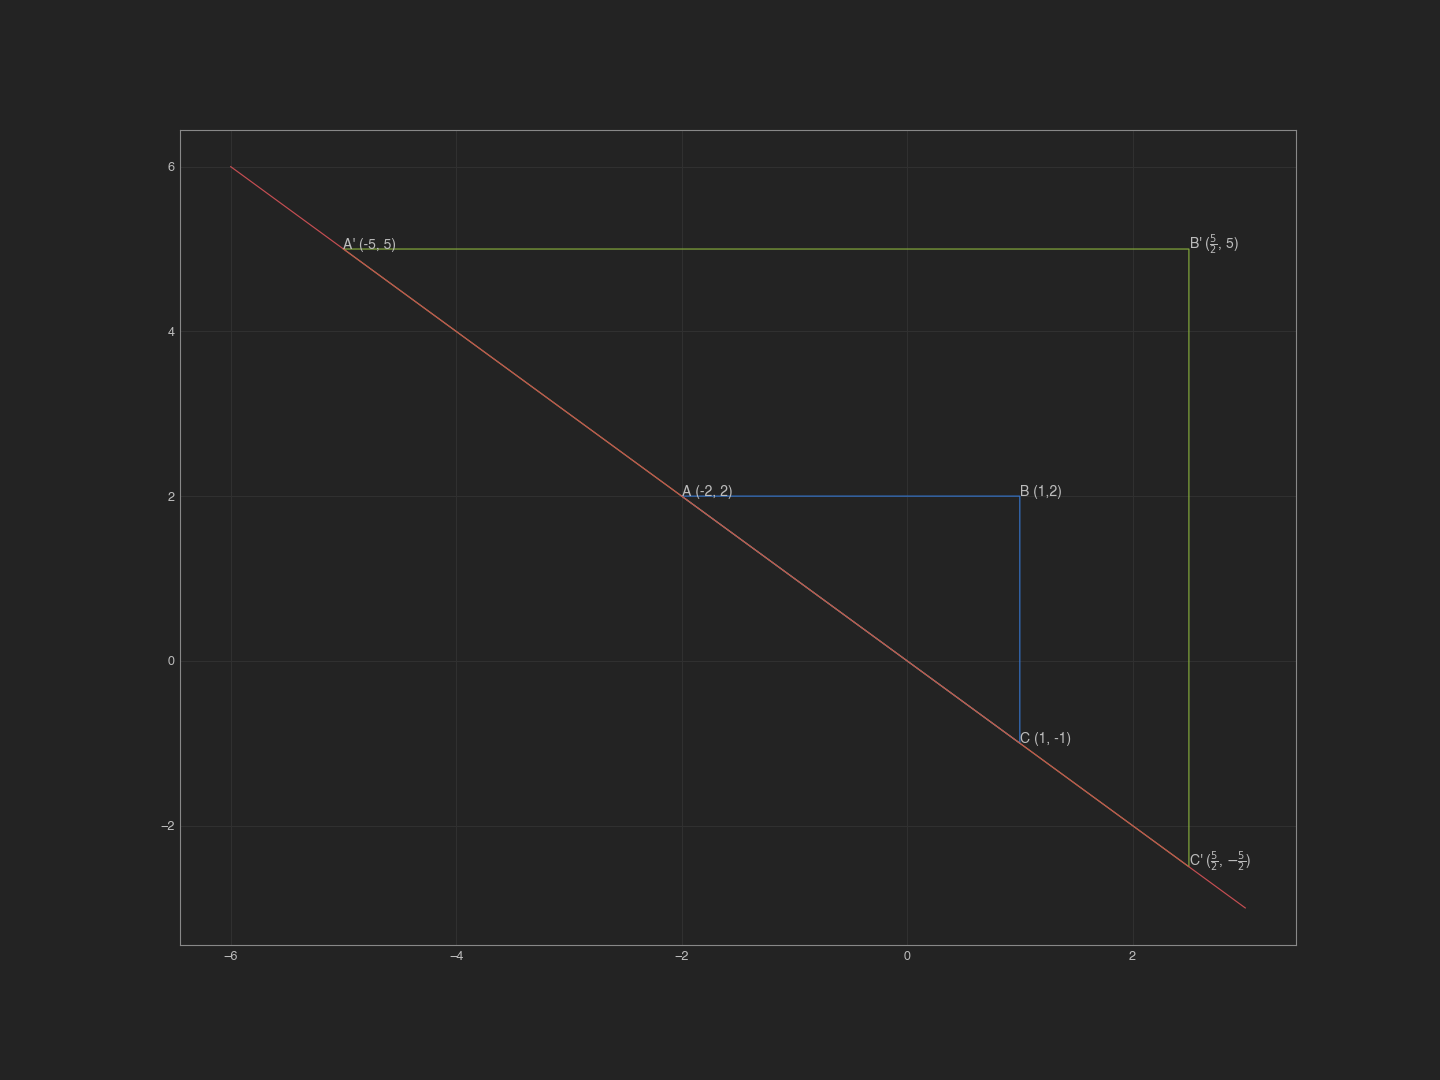
\includegraphics[width=1.0\columnwidth]{dilation}
  \caption{Pre Image and Image of Triangle}
\end{figure}
The equation of the line is :
\begin{align}
  C (1, -1) , O (0,0) \\
  m = \frac{0 -1}{0 + 1} \\
  y = -x + b \rightarrow 2 = 2 + b \rightarrow b = 0 \\
  y = -x
\end{align}
\end{center}
\end{document}
